\chapter{METHODOLOGY}
\label{chap:methodology}

\section{Introduction}

\hs This chapter describes the experimental design, data acquisition, model development, and evaluation procedures implemented during the internship project. The primary objective is to develop a robust and deployable deep learning framework for the automatic detection and pixel-level segmentation of cracks in large-scale, high-resolution aerial imagery captured by Unmanned Aerial Vehicles (UAVs) \cite{01-zhang-2024a, 07-chen-2024}. The methodology has been designed to address the key technical objectives established in Chapter 1:

\begin{itemize}
    \item \textbf{Unify and standardize multiple public crack datasets} to construct a diverse and balanced data pool for model training.
    \item \textbf{Develop and evaluate multiple state-of-the-art architectures} across semantic segmentation, instance segmentation, and transformer-based paradigms.
    \item \textbf{Design and implement a tile-based inference pipeline with blended overlaps} to enable the seamless processing of arbitrarily large-scale images on a single Graphics Processing Unit (GPU).
    \item \textbf{Validate the pipeline on a custom, high-resolution self-collected UAV dataset} to verify its real-world robustness.
\end{itemize}

\section{Data Acquisition}
\label{sec:data_acquisition}

\hs To train a robust and generalizable deep learning model, a diverse collection of data is required. This section details the curation of public benchmarks, the collection protocol of our custom UAV dataset, and the preprocessing steps established to unify these disparate sources.

\subsection{Public Datasets}
\label{subsec:public-datasets}

\hs To build a diverse and robust training corpus, we aggregated publicly available crack detection datasets curated in the GitHub repository \textbf{Cv-learning/Crack-Dataset}. This repository consolidates multiple benchmark datasets from the literature, providing a unified collection of crack images with corresponding pixel-level annotations.

\newpage

\hs The combined dataset comprises 8,818 RGB images and their binary segmentation masks, covering a wide variety of crack morphologies, surface materials (concrete, asphalt, brick, etc.), and imaging conditions (different lighting, shadows, and viewing angles). The specific datasets included in this aggregation are those listed in the repository’s documentation, which bring together well-known benchmarks such as CFD, Crack500, DeepCrack, Tunnel Crack, and other sources as indicated in the repository. All images were resampled to a consistent resolution and paired with their ground-truth masks.

\begin{table}[htbp]
    \centering
    \setlength{\tabcolsep}{5pt}
    \caption{\textit{Detailed specifications of the constituent public crack datasets.}}
    \label{tab:constituent_datasets}
    \begin{tabularx}{\textwidth}{l l X X}
        \toprule
        \textbf{Dataset}      & \textbf{Images} & \textbf{Surface}                   & \textbf{Academic Citation}             \\
        \midrule
        \textbf{CFD}          & 118             & Asphalt pavement                   & Shi et al. (2016) \cite{28-shi-2016}      \\
        \addlinespace
        \textbf{Crack500}     & 500             & Concrete pavements                 & Zhang et al. (2016) \cite{08-zhang-2016}  \\
        \addlinespace
        \textbf{DeepCrack}    & 537             & Cement, asphalt, and concrete      & Liu et al. (2019) \cite{03-liu-2019}   \\
        \addlinespace
        \textbf{Tunnel Crack} & \textbf{7,663}  & Concrete tunnel walls              & CV-learning Repository\footnotemark[1] \\
        \midrule
        \textbf{Total}        & \textbf{8,818}  & \textbf{Mixed structural surfaces} & \textbf{Combined Dataset}              \\
        \bottomrule
    \end{tabularx}
\end{table}

\subsection{CUBIT-InSeg Large-Scale UAV Dataset}
\label{sebsec:cubit-for-zero-shot}

\hs CUBIT-InSeg was used exclusively as an external, unseen test set and was not included in the training or validation splits. This decision reflects the deployment context of the project as the models' performance is intended to be delivered to a niche customer whose UAV-captured imagery and implementation environments will differ from any public benchmark. The first deployment to a new customer site is therefore inherently a zero-shot scenario, and CUBIT-InSeg provides a realistic proxy for that condition.

\hs Fine-tuning on CUBIT-InSeg was deliberately avoided. In the intended workflow, fine-tuning is reserved as a deployment-time adaptation step, in which the model is retrained on a small set of images collected from the customer's own environment. Performing fine-tuning on CUBIT-InSeg during development would have consumed this adaptation step on a dataset that is not the customer's, and would have obscured the model's true zero-shot generalization performance. The CUBIT-InSeg results in Section \ref{sec:results_and_analysis_on_large_scale_images}; therefore represent a conservative estimate of the model's expected performance after customer-specific fine-tuning.

\hs This zero-shot protocol is maintained for all three models to ensure a fair comparison. Any subsequent fine-tuning would be performed only on data collected from the target deployment site.

\footnotetext[1]{Retrieved from: \url{https://github.com/Cv-learning/Crack-Dataset}.}

\newpage

\subsection{Planned Self-Collected UAV Dataset}

\hs To complement the public benchmarks with real-world aerial imagery, a custom UAV-based crack dataset was proposed for collection by the Drone Operations Department at AI Farm Robotics. The intended acquisition protocol specified flights at an altitude of 10–15 m using a high-resolution RGB sensor, targeting building facades and rooftops in Phnom Penh, with annotations to be performed manually by trained technicians.

\hs However, at the time of this internship (July–September 2026), the data collection and annotation pipeline had not been completed by the Drone Operations Department. Consequently, this dataset was not available for integration into the training, validation, or testing phases of the current study.

\hs The absence of this dataset does not invalidate the experimental framework, as the aggregated public datasets (Section~\ref{subsec:public-datasets}) provide a sufficiently diverse and challenging benchmark covering multiple surface types, lighting conditions, and crack morphologies. Validation on genuine UAV-captured imagery remains an important direction for future work, contingent on the completion of the data collection effort by the drone team.

\section{Data Preparation}

\subsection{Annotation Unification and Standardization}

\hs To make all training data compatible, the annotation formats from different sources were converted into a common binary pixel representation. Each ground-truth label was transformed into a single-channel mask, where the mathematical definition is:

\begin{equation}
    M(x, y) = \begin{cases}
        1, & \text{if pixel } (x, y) \text{ belongs to a crack region} \\
        0, & \text{otherwise (background)}
    \end{cases}
\end{equation}

\hs For practical storage, these binary masks were saved as 8-bit single-channel PNG files. In this format, a pixel value of \textbf{255 (white)} represents a crack, corresponding to the mathematical value $1$, while a pixel value of \textbf{0 (black)} represents the background, corresponding to the mathematical value $0$. During data loading, the pixel values are normalized by dividing by 255 to recover the $\{0,1\}$ representation used for model training and loss computation. This dual representation, mathematical $\{0,1\}$ for computation and $\{0,255\}$ for storage, is standard practice in image segmentation and ensures compatibility with both deep learning frameworks and standard image I/O libraries.

\newpage

\begin{figure}[htbp]
    \centering
    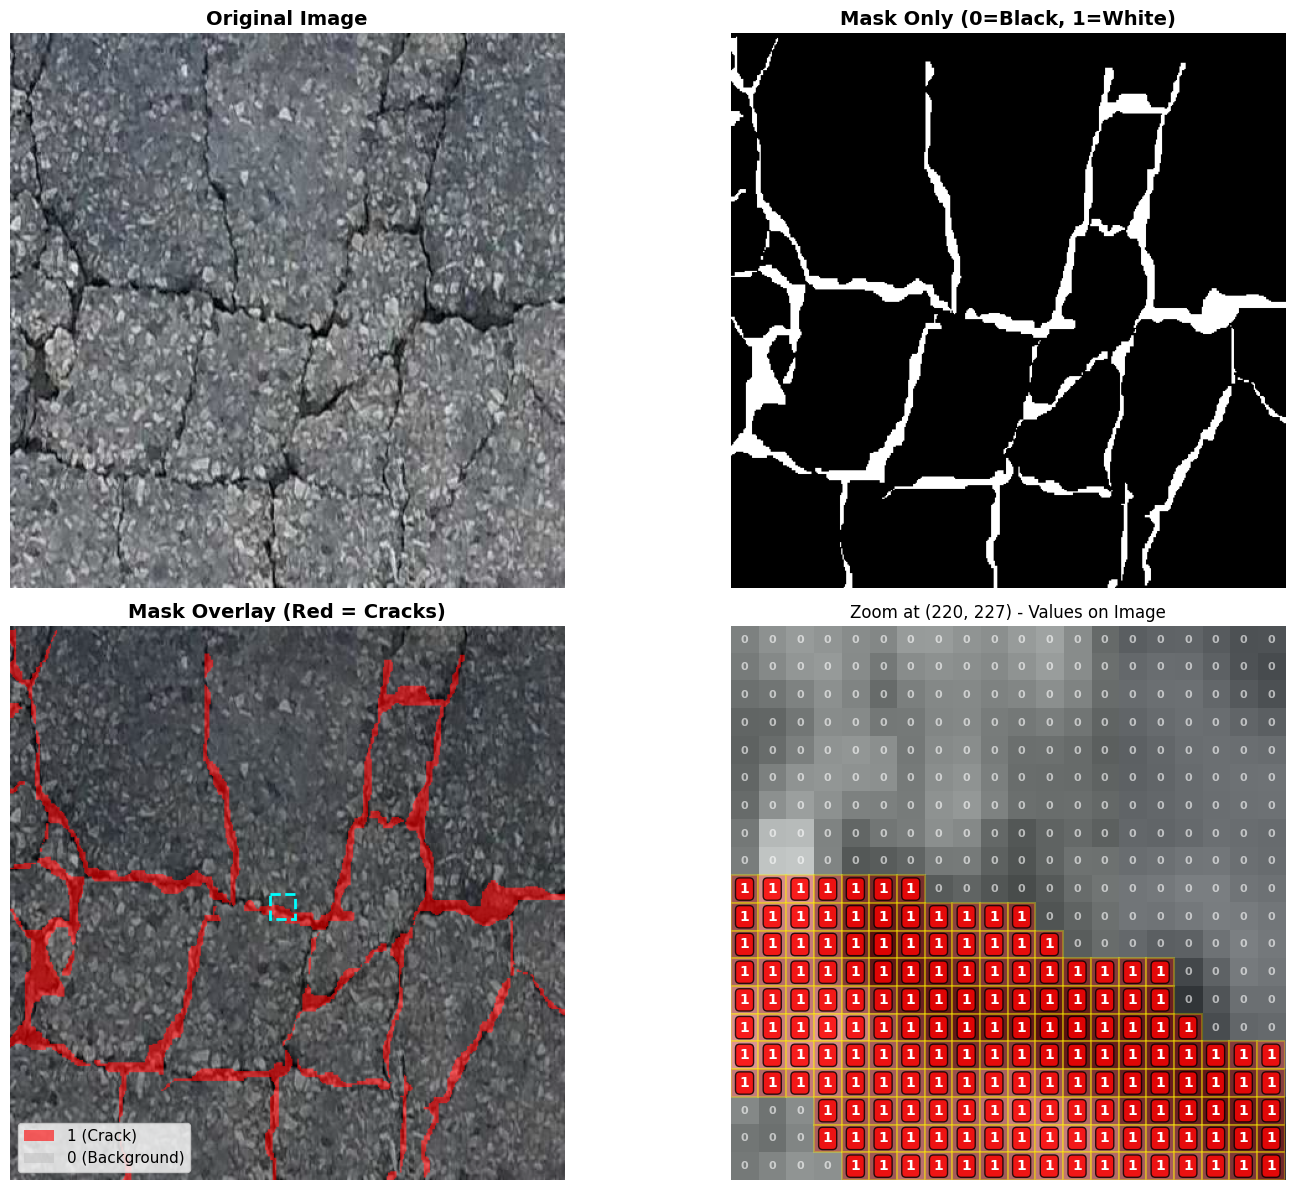
\includegraphics[width=\linewidth]{figures/cracks/crack-map.png}
    \caption{\textit{Binary pixel-level annotation used for model training and evaluation.}}
    \label{fig:crack_map}
\end{figure}

\hs This unified annotation scheme ensures consistent processing across all datasets. The binary representation simplifies loss computation and metric calculation while preserving pixel-level spatial precision.

\hs Because all masks follow the same binary convention, they can be loaded with standard image libraries and passed directly to the loss functions without any format-specific preprocessing. This uniformity is essential when training on images drawn from multiple sources, where annotation styles and class definitions may otherwise differ. It also allows the same evaluation metrics to be applied consistently across every dataset in the study. Maintaining a single annotation format therefore removes a common source of training instability that arises when labels from different sources are combined without normalization. This step is particularly important for crack segmentation, where differences in how crack edges are annotated can otherwise introduce systematic bias into the learned decision boundary.

\newpage

\subsection{Patch Extraction and Sliding Window Strategy}
\label{subsec:patch_extract_slicing_window}

\hs To accommodate images of varying resolutions within a unified training and inference pipeline, all source images and their corresponding binary masks were decomposed into fixed-size tiles of \(512 \times 512\) pixels.

\textbf{Training Phase}

\hs All training images were sourced exclusively from the public crack datasets described in Section~\ref{subsec:public-datasets}. These images have a native resolution of \(448 \times 448\) pixels. To standardize inputs for batch processing, symmetric zero-padding was applied to the boundaries to reach the target size of \(512 \times 512\) pixels, as illustrated in Figure~\ref{fig:training_image_resize}. This padding ensures that the spatial aspect ratio is preserved without distorting the crack features.

\begin{figure}[htbp]
    \centering
    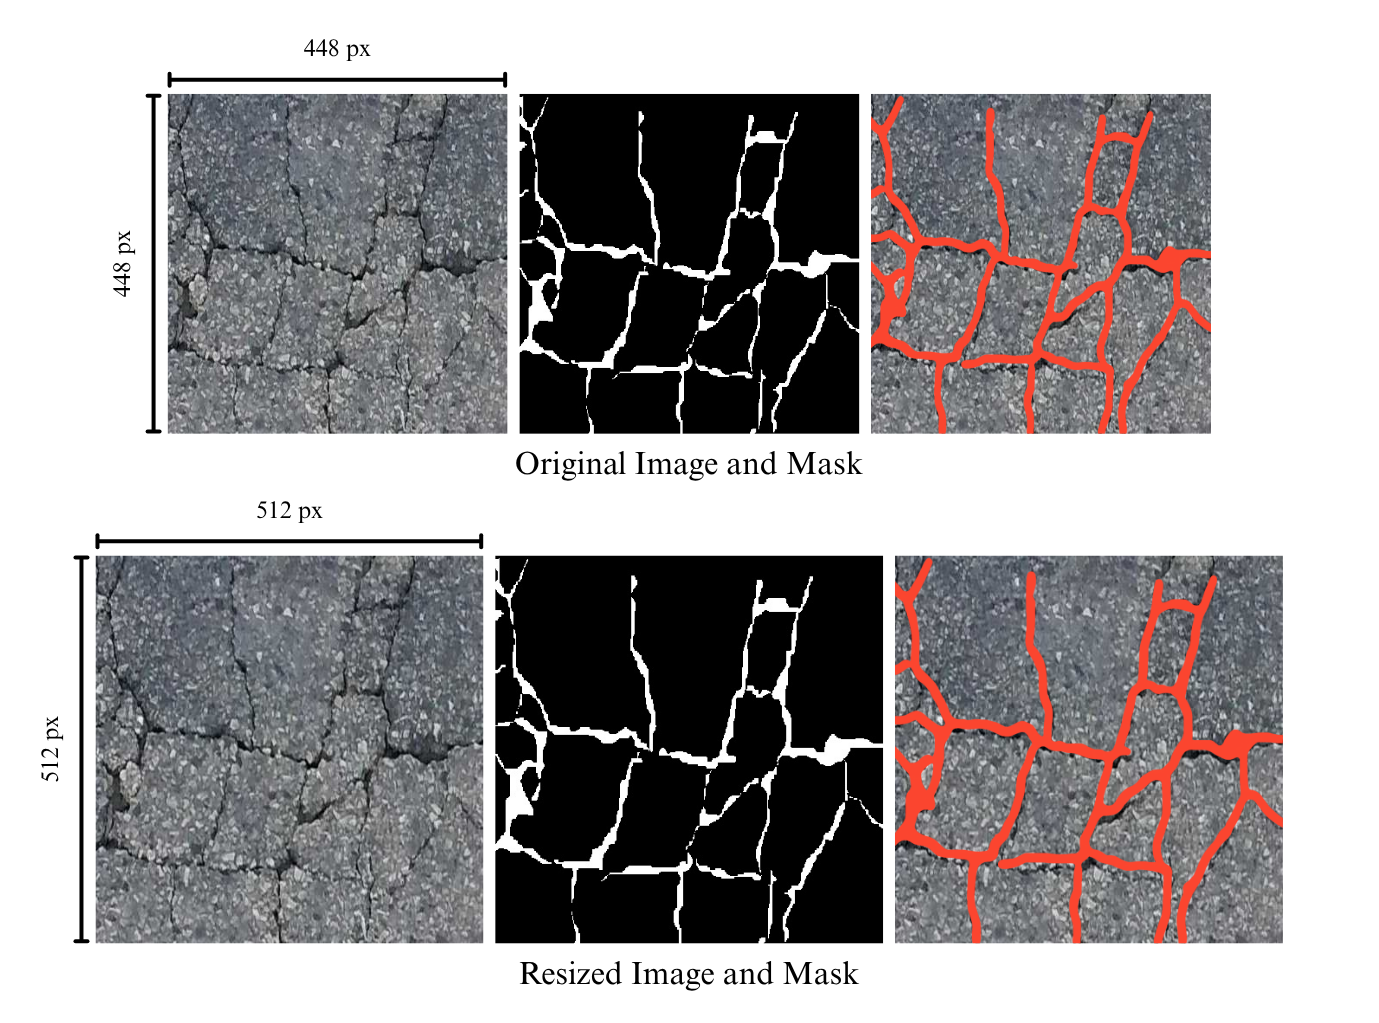
\includegraphics[width=\linewidth]{figures/cracks/image-resizing.png}
    \caption{\textit{Padding for training images, showing the symmetric zero-padding applied to reach the target size of \(512 \times 512\) pixels.}}
    \label{fig:training_image_resize}
\end{figure}

\hs Zero-padding was chosen over resizing because interpolation would distort the crack geometry and blur the thin, high-frequency edges that the models must learn to detect. Although the padded border contains no useful signal, it is masked out during loss computation, so the network never receives gradient updates from these regions. This keeps training stable while preserving the original appearance of every crack.

\newpage

\textbf{Inference Phase}

\hs For high-resolution inference, the sliding window strategy was designed to process arbitrarily large images that exceed GPU memory limits. The window size was set to \(512 \times 512\) pixels with a stride of 384 pixels, corresponding to a 128-pixel overlap (25\%) in both horizontal and vertical directions.

\begin{figure}[htbp]
    \centering
    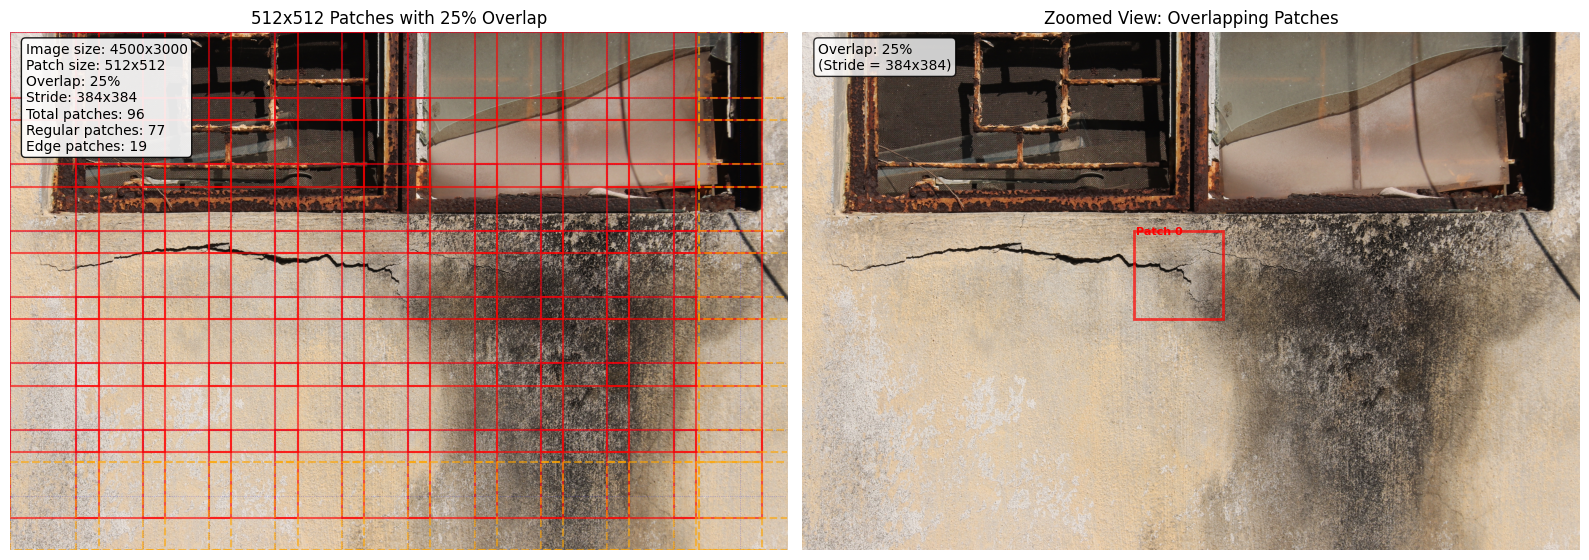
\includegraphics[width=\linewidth]{figures/cracks/inference-patching.png}
    \caption{\textit{Sliding window for high-resolution inference, showing the overlap between adjacent patches.}}
    \label{fig:inference_patching}
\end{figure}

\hs This overlap ensures that cracks located near tile boundaries are not truncated or lost during independent tile forward passes.

\hs The inference pipeline was validated on high-resolution test images of approximately 13.5 megapixels, which were sourced from the public datasets' test split (where native resolutions exceeded \(512 \times 512\)) and used exclusively for evaluation. These images, while not reaching the gigapixel scale targeted for final deployment, were sufficiently large to demonstrate the effectiveness of the tile-based approach and the blended overlap merging strategy. The pipeline is architecturally scalable to gigapixel images, as the tile processing is independent of total image dimensions, requiring only sufficient disk storage and sequential processing.

\begin{figure}[htbp]
    \centering
    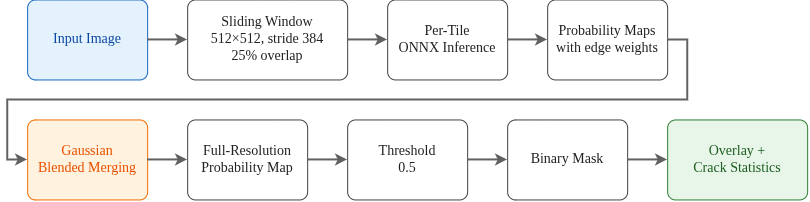
\includegraphics[width=\linewidth]{figures/cracks/tile_pipeline.png}
    \caption{\textit{Blended overlap merging strategy for reconstructing the full probability map from overlapping tiles.}}
    \label{fig:overlap_merging}
\end{figure}

\newpage

\hs If an input image's dimensions are not perfectly divisible by the stride, zero-padding is temporarily applied to the right and bottom boundaries. After the blended overlap merging reconstructs the full probability map, the padded regions are cropped back to the original image dimensions.

\begin{table}[h]
    \centering
    \caption{\textit{Summary of patch extraction and sliding window parameters}}
    \label{tab:patch_parameters}
    \renewcommand{\arraystretch}{1.1}
    \begin{tabular}{@{}l c@{}}
        \toprule
        \textbf{Parameter}                     & \textbf{Value}            \\
        \midrule
        Training image size (before padding)   & \(448 \times 448\) pixels \\
        Training patch size (after padding)    & \(512 \times 512\) pixels \\
        Inference patch size                   & \(512 \times 512\) pixels \\
        Inference overlap                      & 128 pixels (\(25\%\))     \\
        \textit{UAV image size (Generalization Test)} & \textit{>10 megapixels}            \\
        \bottomrule
    \end{tabular}
\end{table}

\subsection{Dataset Splitting}
\label{subsec:dataset_splitting}

\hs To ensure fair and unbiased evaluation, the entire set of 8,818 images was 
divided strictly at the image level into three disjoint subsets.

\hs Splitting was performed at the source-image level rather than at the 
patch level. This is a critical design choice: if tiles from the same source 
image were allowed to appear in both the training and test splits, the model 
would effectively be evaluated on data it had already seen, since adjacent 
tiles often share overlapping content, lighting conditions, and surface 
texture. By enforcing image-level separation, no tile in the test set shares 
its parent image with any tile in the training set.

\begin{table}[htbp]
    \centering
    \caption{\textit{Summary of public crack dataset partition.}}
    \label{tab:dataset_split}
    \renewcommand{\arraystretch}{1.1}
    \resizebox{\textwidth}{!}{%
        \begin{tabular}{lccc l}
            \toprule
            \textbf{Dataset Split} & \textbf{Split Percentage (\%)} & \textbf{Paired Image Count} & \textbf{Role in Training Pipeline}                 \\
            \midrule
            Training               & 80\%                           & 7,054                       & Active gradient optimization \& backpropagation    \\
            Validation             & 10\%                           & 882                         & Hyperparameter selection \& overfitting prevention \\
            Testing                & 10\%                           & 882                         & Independent, unseen benchmark evaluation           \\
            \midrule
            \textbf{Total}         & \textbf{100\%}                 & \textbf{8,818}              & \textbf{Comprehensive Compiled Public Database}    \\
            \bottomrule
        \end{tabular}%
    }
\end{table}

\hs By enforcing source-image level splitting, tiles from the same physical 
road section or lighting condition were prevented from appearing in both the 
training and evaluation splits. This ensures that reported performance 
reflects generalization to unseen surfaces rather than memorization of 
specific source images, mirroring the intended deployment scenario.

\hs The three-way split described in Table \ref{tab:dataset_split} applies 
to the aggregated public dataset only. The CUBIT-InSeg dataset, described in 
Section \ref{sebsec:cubit-for-zero-shot}, is deliberately excluded and used 
as an external zero-shot test set.

\newpage

\subsection{Class Imbalance Analysis}
\label{subsec:class_imbalance_analysis}

\hs \hs An analysis of pixel-level class distribution in the training set revealed 
significant class imbalance. Figure \ref{fig:class_distribution} summarizes the 
exact counts and their visual proportions, showing that crack pixels account for 
76,705,349 of the 2,382,523,973 total pixels (3.33\%), while background pixels 
account for the remaining 2,305,818,624 pixels (96.67\%). This corresponds to 
an approximate 32:1 background-to-crack ratio.

\begin{figure}[htbp]
    \centering
    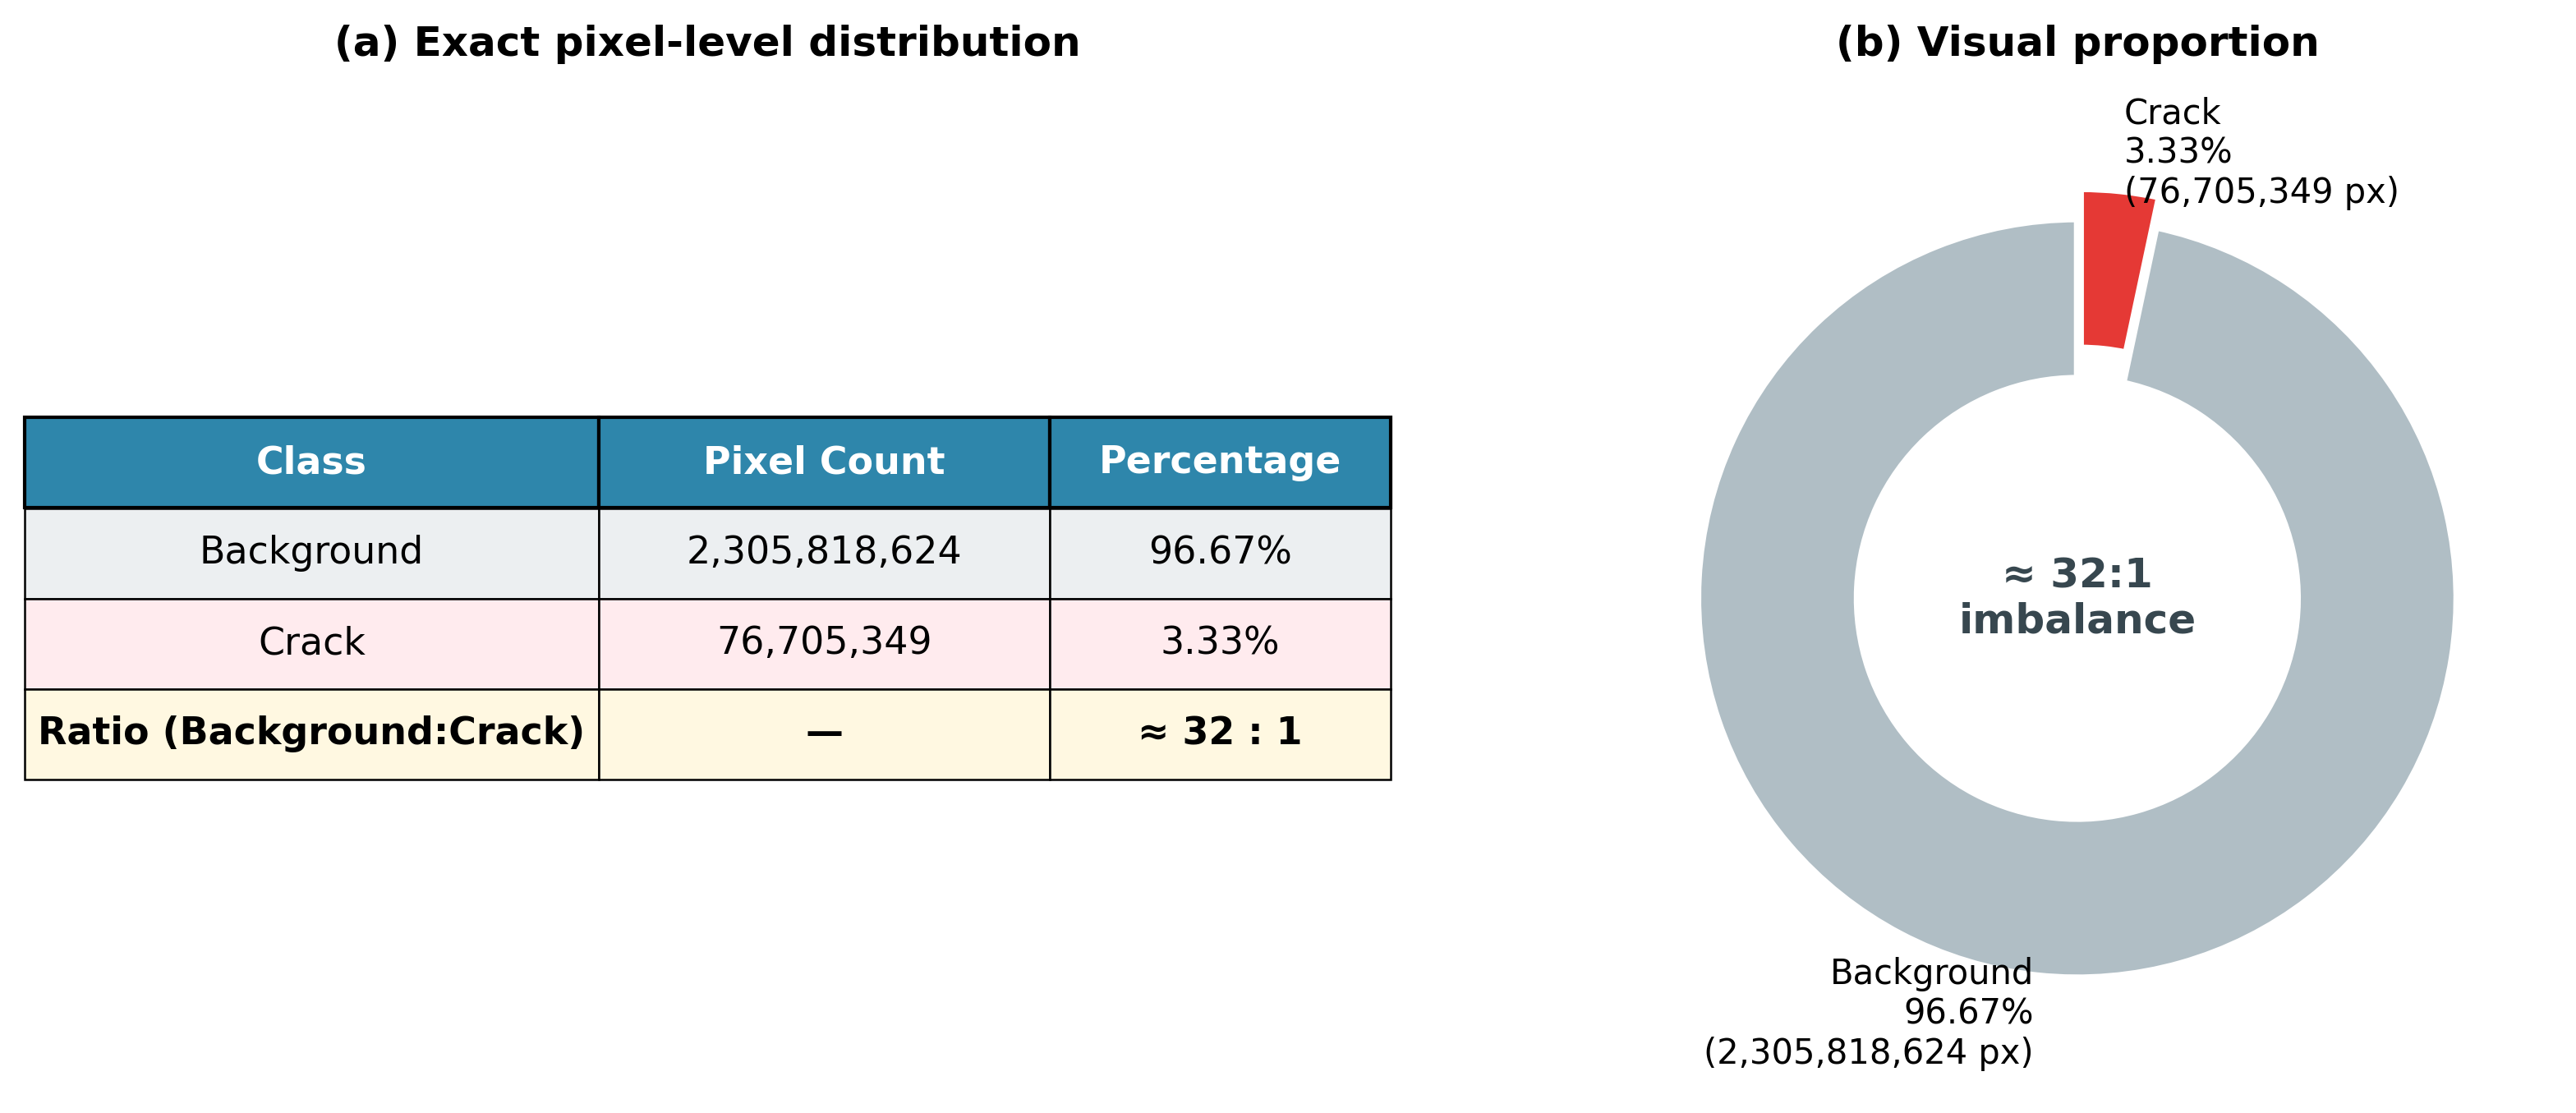
\includegraphics[width=\textwidth]{figures/plots/class_distribution_merged (Edited).png}
    \caption{\textit{Pixel-level class distribution in the training dataset.}}
    \label{fig:class_distribution}
    
\end{figure}

\hs Two practical consequences follow from this distribution. First, standard 
cross-entropy loss functions, which weight each pixel equally, are dominated by 
the background class and tend to produce models that predict crack pixels poorly, a phenomenon confirmed during preliminary experiments and addressed in 
Section \ref{subsec:loss_functions} through the combined loss strategy. Second, 
pixel accuracy is an inappropriate evaluation metric for this task: a naive 
model that predicts background for every pixel would achieve 96.67\% accuracy 
while detecting no cracks at all. For this reason, evaluation throughout this 
study relies on IoU, F1-score, and recall, which measure positive-class 
performance directly, as detailed in Section \ref{subsec:evaluation_metrics}.

\section{Model Development and Selection}
\label{sec:model_development_and_selection}

\hs To empirically evaluate the trade-offs between accuracy, inference speed, and spatial context-awareness, three distinct families of state-of-the-art segmentation architectures were selected and evaluated. While the baseline architectures are well-established in the literature (Section \ref{sec:deep_learning_models}), specific modifications were applied to U-Net and SegFormer to address the unique challenges of crack segmentation, particularly extreme class imbalance and the need to preserve fine, thread-like structures. YOLO26s-seg was evaluated using its native configuration without architectural modification to serve as a deployment-oriented baseline.

\newpage

\subsection{Selection Rationale}
\label{subsec:selection_rationale}

The choice of architectures was guided by three primary considerations:

\begin{itemize}
    \item \textbf{Architectural diversity:} To compare fundamentally different approaches to segmentation (CNN-based semantic segmentation, CNN-based instance segmentation, and transformer-based segmentation).
    \item \textbf{Deployability:} All selected models are lightweight enough for edge-device deployment, a key requirement for the internship's focus on practical robotics applications at AI Farm Robotics.
    \item \textbf{Proven performance:} Each architecture has demonstrated strong performance on crack detection or similar fine-structure segmentation tasks in the literature.
\end{itemize}

\begin{table}[h]
    \centering
    \caption{\textit{Comparison of selected model architectures.}}
    \label{tab:model_comparison}
    \renewcommand{\arraystretch}{1.2}
    \resizebox{\textwidth}{!}{%
        \begin{tabular}{@{}l l c c c@{}}
            \toprule
            \textbf{Model Family} & \textbf{Backbone} & \textbf{Params (M)} & \textbf{FLOPs (G)} & \textbf{Key Feature}                         \\
            \midrule
            U-Net                 & EfficientNet-B0   & 6.30                & 12.0               & Skip connections preserve fine crack details \\
            SegFormer             & MiT-B0            & 3.71                & 7.87               & Global receptive field via self-attention    \\
            YOLO                  & YOLO26s-seg       & 11.43               & 34.3               & Single-stage, instance-level output          \\
            \bottomrule
        \end{tabular}%
    }
\end{table}

\subsection{Baseline Architectures}
\subsubsection{Semantic Segmentation: U-Net}
\hs U-Net was selected as the primary semantic segmentation baseline due to its established performance in crack detection. The architecture employs a symmetric encoder-decoder structure with skip connections that directly transfer high-resolution local features from the encoder to the decoder. This design is particularly beneficial for thin crack detection, as it preserves fine spatial details that are often lost in deeper networks.

\textbf{Architectural Modifications:}

\hs The baseline U-Net was adapted using the Segmentation Models PyTorch (SMP) framework with the following changes:

\begin{enumerate}
    \item \textbf{EfficientNet-B0 Encoder:} The default U-Net encoder was replaced with an EfficientNet-B0 backbone pre-trained on ImageNet (See Table \ref{tab:model_comparison}). With only 6.3 million total parameters, this encoder balances computational efficiency with strong feature extraction performance, making it suitable for deployment on resource-constrained edge devices. The encoder weights were initialized from ImageNet pre-training and fine-tuned end-to-end during training.

    \item \textbf{Spatial and Channel Squeeze-and-Excitation (scSE) Attention:} The U-Net decoder incorporates scSE attention modules, configured with a scSE decoder attention setting\footnote{Set in code: \texttt{decoder\_attention\_type=``scse''}}, to refine feature representations and improve detection of subtle crack patterns. The scSE mechanism recalibrates channel-wise and spatial feature responses, allowing the network to focus on informative regions while suppressing irrelevant background textures, a critical capability when cracks occupy less than 1\% of the image area.

    \item \textbf{Combined Loss Function:} A weighted combination of Binary Cross-Entropy (BCE), Dice, and Focal losses was employed (see Section \ref{subsec:loss_functions}). This is a departure from the original U-Net formulation, which used pixel-wise softmax with cross-entropy \cite{30-ronneberger-2015-unet}.
\end{enumerate}

\begin{figure}[H]
    \centering
    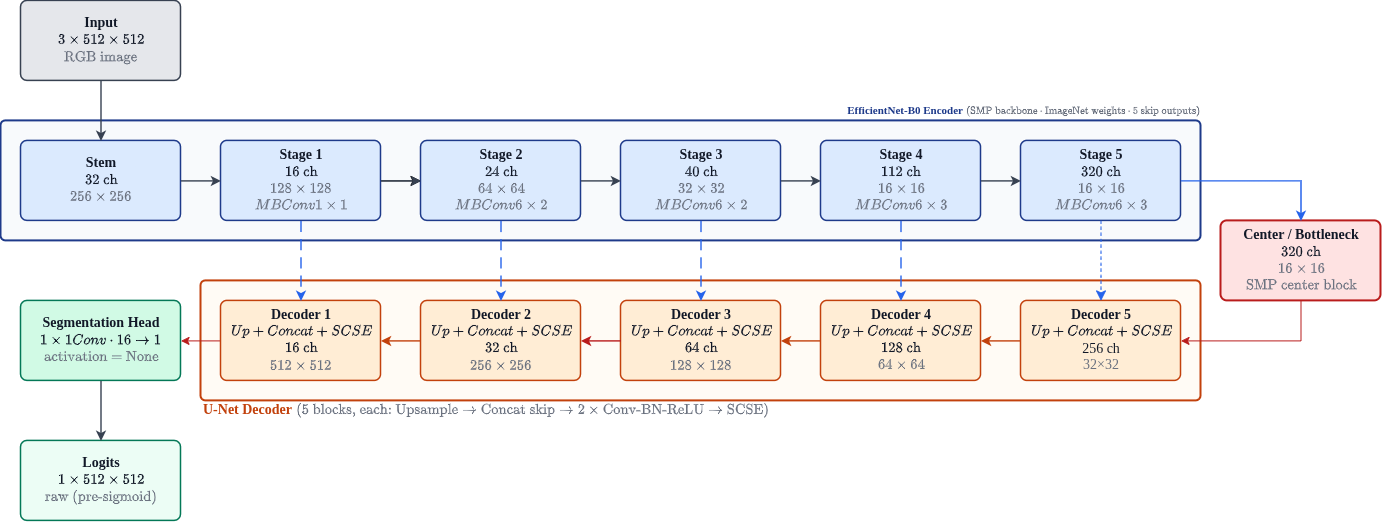
\includegraphics[width=\textwidth]{figures/architectures/unet-architecture.png}
    \caption{\textit{Modified U-Net Architecture.}}
    \label{fig:unet-modified}
\end{figure}

\textit{Illustration of the modified U-Net architecture.} The EfficientNet-B0 encoder replaces the original contracting path, while the scSE attention modules are inserted at each decoder stage to recalibrate features before concatenation with skip connections. With injected attention and a combined loss function, the modified U-Net is optimized for the detection of fine, low-contrast crack structures in high-resolution aerial imagery.

\textbf{Strengths:} Superior preservation of fine spatial details; well-established performance on crack segmentation; computationally efficient.

\textbf{Weaknesses:} Limited global receptive field; may struggle with contextual understanding in complex scenes.

\subsubsection{Transformer-Based Models: SegFormer}
\hs SegFormer was selected to evaluate the potential benefits of global receptive fields for crack detection. Traditional convolutional neural networks process features locally using fixed receptive fields, which can lead to loss of continuity for long, branching cracks. Transformers, in contrast, employ self-attention mechanisms to model long-range spatial dependencies across the entire image canvas.

\textbf{Architectural Modifications:}

\begin{figure}[H]
    \centering
    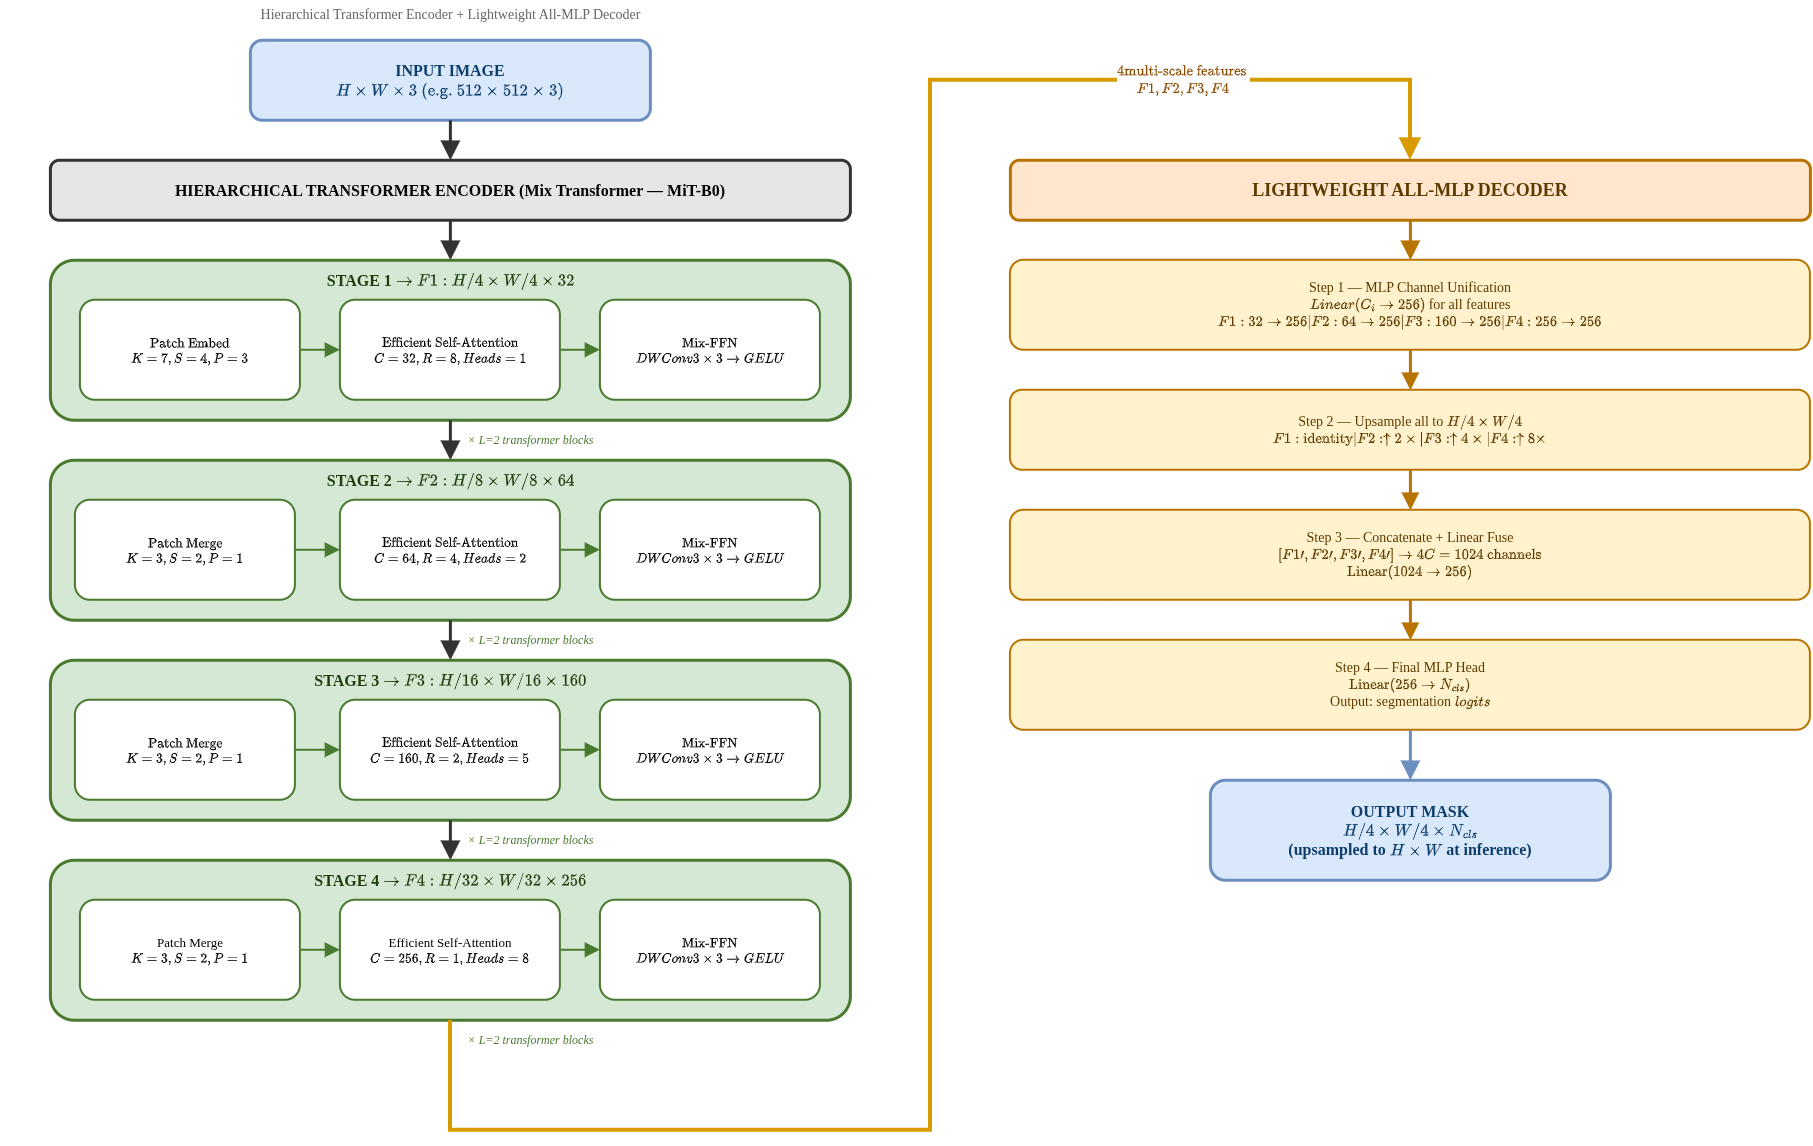
\includegraphics[width=\textwidth]{figures/architectures/segformer-modified.png}
    \caption{\textit{SegFormer Architecture.}}
    \label{fig:segformer-architecture}
\end{figure}

\hs The SegFormer architecture was adapted using the SMP framework with the changes:

\begin{enumerate}
    \item \textbf{Lightweight MiT-B0 Encoder:} The Mix Transformer (MiT-B0) variant was selected for its balance of efficiency and representational capacity. With only 3.7 million parameters, SegFormer-MiT-B0 is the lightest model evaluated in this study (See Table \ref{tab:model_comparison}). The hierarchical encoder captures both high-resolution local details and global contextual features without requiring positional encodings, avoiding performance drops when test resolution differs from training resolution.

    \item \textbf{Combined Loss Function:} A weighted combination of Binary Cross-Entropy (BCE), Dice, and Focal losses was employed (see Section \ref{subsec:loss_functions}). SegFormer's original formulation used cross-entropy loss; the combined loss was introduced to address the extreme foreground-background imbalance in crack detection.

    \item \textbf{Lightweight All-MLP Decoder:} The native SegFormer All-MLP decoder aggregates multi-level features from the hierarchical encoder. By combining local attention from lower layers with global attention from higher layers, the decoder produces powerful representations without computationally expensive modules \cite{32-xie-2021-segformer}.
\end{enumerate}

\textbf{Strengths:} Global receptive field; preserves geometric continuity; lightweight.

\textbf{Weaknesses:} Lacks translational equivariance inductive bias; requires more training data; computationally expensive for self-attention at higher resolutions.

\subsubsection{Instance Segmentation: YOLO}
\label{subsubsec:instance_segmentation_yolo}

\hs YOLO was selected to evaluate whether treating distinct cracks as separate instances reduces noise and improves global delineation. The YOLO family of single-stage, anchor-free detectors is well-suited for real-time edge deployment due to its efficient architecture.

\textbf{Implementation Note:} Unlike U-Net and SegFormer, the YOLO26s-seg model was used with its native architecture and default training configuration as implemented in the Ultralytics framework. No architectural modifications, custom loss functions, or custom augmentation pipelines were applied. This decision was made deliberately to:

\begin{itemize}
    \item Evaluate the out-of-the-box performance of a modern, edge-optimized instance segmentation model on crack detection.

    \item Provide a clean baseline for comparison against the modified semantic and transformer-based models.

    \item Leverage YOLO26's native optimizations, including NMS-free end-to-end inference and DFL removal, which simplify deployment on edge devices \cite{31-sapkota-2026-yolo26}.
\end{itemize}

\hs The YOLO26s-seg variant balances speed and accuracy, incorporating Programmable Gradient Information (PGI) and the Generalized Efficient Layer Aggregation Network (GELAN) to retain spatial details while maintaining low latency. The model outputs both bounding boxes and pixel-level masks, enabling instance-wise analysis of individual cracks. With 11.4 million parameters and 34.3 GFLOPs (See in Table \ref{tab:model_comparison}), YOLO26s-seg is the heaviest model evaluated in this study but offers the advantage of distinguishing individual crack instances and the fastest inference speed \cite{31-sapkota-2026-yolo26}.

\hs Because no custom losses were applied, this model also serves as a reference point for evaluating whether the combined loss objective used by the other models provides a measurable benefit under the same data conditions. Any accuracy gap observed between YOLO26s-seg and the SMP-based models can therefore be attributed partly to the loss design.

\begin{figure}[H]
    \centering
    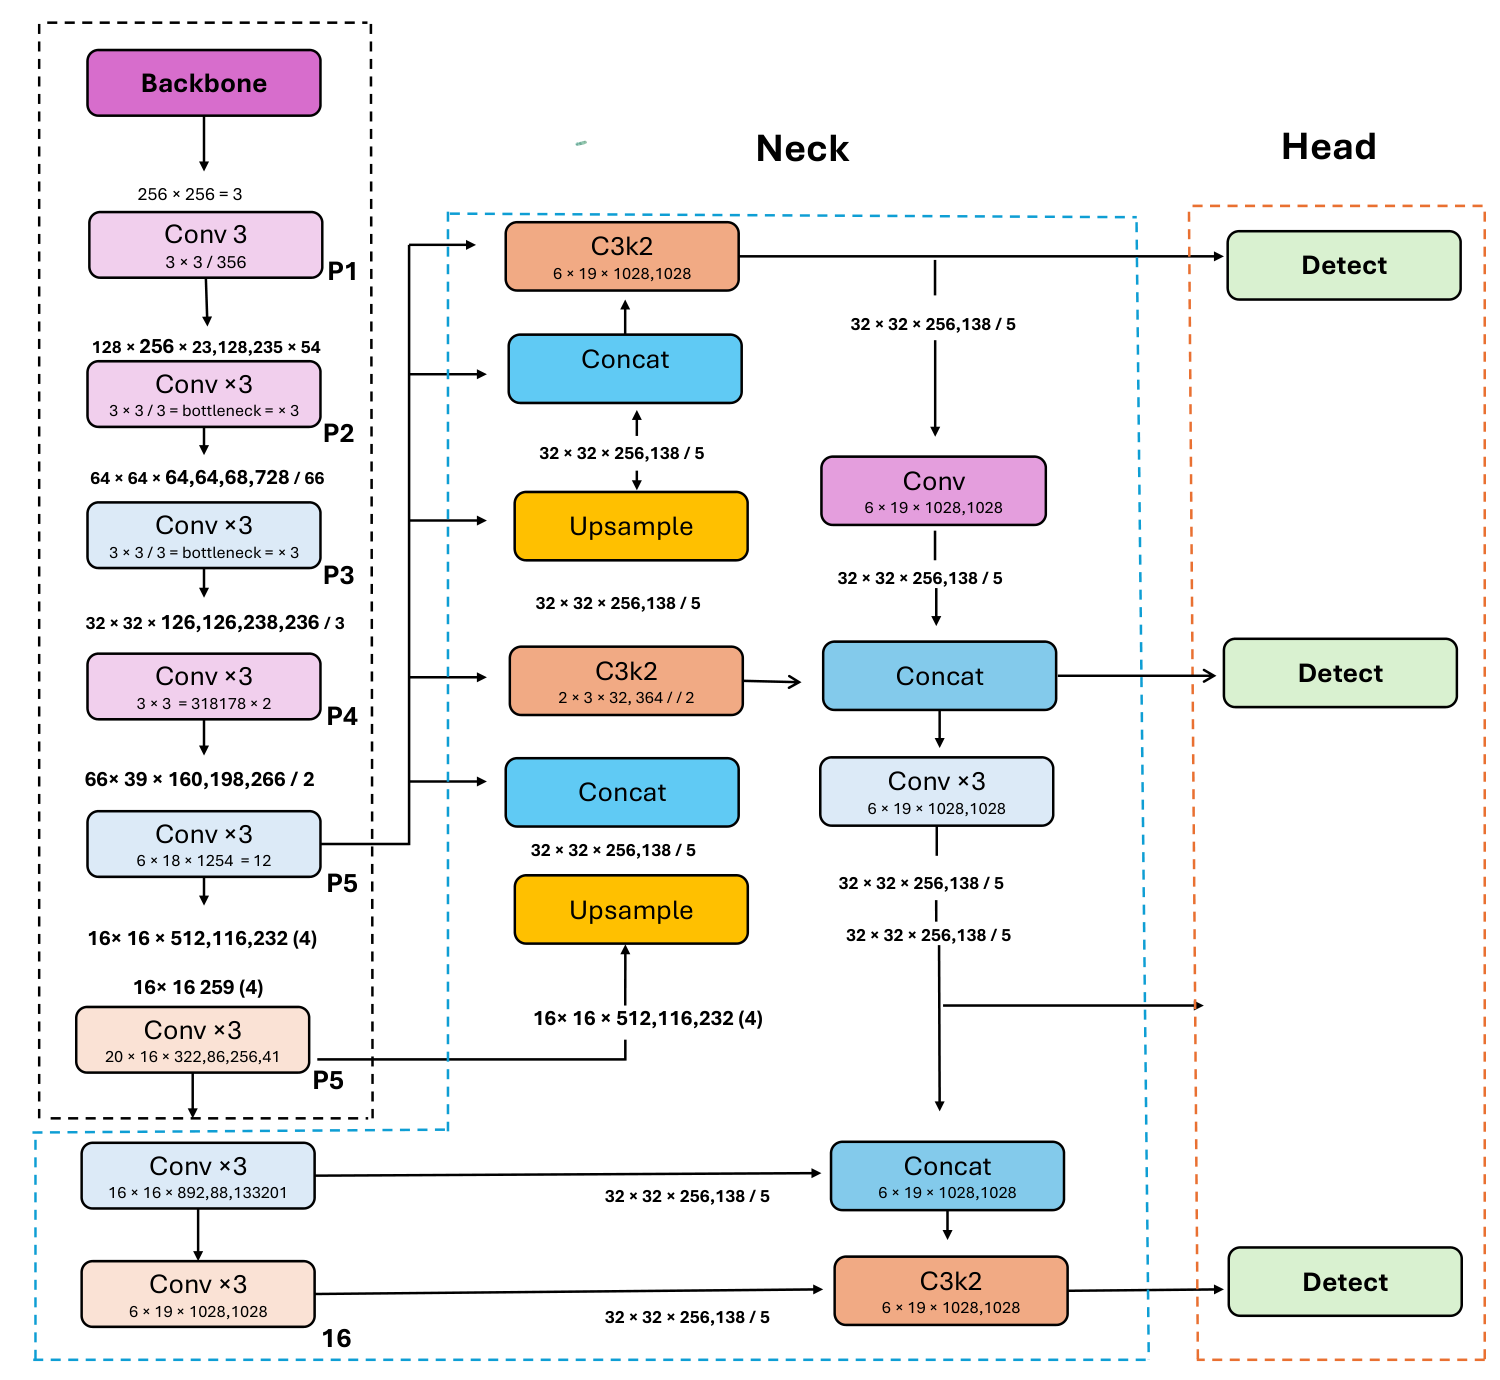
\includegraphics[width=\textwidth]{figures/architectures/yolo26-original.png}
    \caption{\textit{Original YOLO26 Architecture.}}
    \label{fig:yolo26-original}
\end{figure}

\textbf{Strengths:} Fast inference; instance-level differentiation; native NMS-free inference; suitable for real-time edge deployment.

\textbf{Weaknesses:} May miss very thin cracks; requires careful threshold tuning; higher computational cost than lightweight semantic models.

\subsection{Loss Functions}
\label{subsec:loss_functions}

\hs For U-Net and SegFormer (SMP-based models), a combined loss function was employed to address the extreme class imbalance inherent in crack detection, where crack pixels typically occupy less than 1\% of the total image area. This modification was critical, as standard cross-entropy loss alone proved insufficient for learning fine crack structures.

The total loss is formulated as:
\begin{equation}
    L_{\text{total}} = w_{\text{BCE}} \cdot L_{\text{BCE}} + w_{\text{Dice}} \cdot L_{\text{Dice}} + w_{\text{Focal}} \cdot L_{\text{Focal}}
\end{equation}
where the weights were set to \[w_{\text{BCE}} = 0.3, w_{\text{Dice}} = 0.3, \text{and } w_{\text{Focal}} = 0.4\] for both models, determined through preliminary experiments.

\textbf{Binary Cross-Entropy (BCE) Loss.} BCE provides pixel-wise classification supervision, ensuring each pixel is individually evaluated against the ground truth:
\begin{equation}
    L_{\text{BCE}} = -\frac{1}{N} \sum_{i=1}^{N} \left[ y_i \log(p_i) + (1 - y_i) \log(1 - p_i) \right]
\end{equation}

\textbf{Dice Loss.} Dice loss optimizes the overlap between predicted and ground truth masks, which is more robust to class imbalance than BCE alone. It directly maximizes the F1-score at the pixel level:
\begin{equation}
    L_{\text{Dice}} = 1 - \frac{2 \, |P \cap G|}{|P| + |G|}
\end{equation}
where $P$ and $G$ denote the predicted and ground truth masks, respectively.

\textbf{Focal Loss.} Focal loss \cite{29-lin-2017-focal-loss} down-weights the contribution of well-classified examples, forcing the model to focus on hard-to-classify crack pixels:
\begin{equation}
    L_{\text{Focal}} = -\frac{1}{N} \sum_{i=1}^{N} (1 - p_i)^{\gamma} \, y_i \log(p_i)
\end{equation}
A focusing parameter of $\gamma = 2.0$ was used as recommended by \cite{29-lin-2017-focal-loss}. The Focal Loss is particularly effective for crack segmentation because it prevents the vast number of easy-to-classify background pixels from overwhelming the training signal.

\textbf{For YOLO:} YOLO employs its native loss function as implemented in the Ultralytics framework. The loss comprises multiple components:
\begin{equation}
    L_{\text{YOLO}} = L_{\text{box}} + L_{\text{cls}} + L_{\text{dfl}} + L_{\text{mask}}
\end{equation}

where:

\begin{itemize}
    \item $L_{\text{box}}$ is the bounding box regression loss (CIoU loss).
    \item $L_{\text{cls}}$ is the classification loss for object presence.
    \item $L_{\text{dfl}}$ is the Distribution Focal Loss for improved localization.
    \item $L_{\text{mask}}$ is the binary segmentation loss for mask prediction.
\end{itemize}

\hs This multi-component loss enables YOLO to jointly optimize detection and segmentation in a single-stage pipeline. No custom loss modifications were applied to YOLO in this study \cite{31-sapkota-2026-yolo26}.

\subsection{Training Configuration Summary}
\label{subsec"training_config_summary}

Table~\ref{tab:training-hyperparameters} summarizes the training hyperparameters used for each model.

\begin{table}[htbp]
    \centering
    \caption{\textit{Training hyperparameters by model}}
    \label{tab:training-hyperparameters}
    \scriptsize
    \setlength{\tabcolsep}{3pt}
    \begin{tabularx}{\textwidth}{lXXX}
        \hline
        \textbf{Parameter}    & \textbf{U-Net (EfficientNet-B0)}                              & \textbf{SegFormer (MiT-B0)}                                   & \textbf{YOLO26s-seg}           \\
        \hline
        Framework             & SMP (PyTorch)                                                 & SMP (PyTorch)                                                 & Ultralytics                    \\
        Input size            & $512 \times 512$                                              & $512 \times 512$                                              & $512 \times 512$               \\
        Batch size (train)    & 16                                                            & 8                                                             & 32                             \\
        Batch size (val)      & 8                                                             & 8                                                             & 32                             \\
        Epochs (max)          & 50                                                            & 50                                                            & 200 (early stop at 92)         \\
        Optimizer             & AdamW                                                         & AdamW                                                         & MuSGD (auto)                   \\
        Learning rate         & $10^{-3}$                                                     & $10^{-4}$                                                     & 0.01 (auto)                    \\
        Weight decay          & $10^{-4}$                                                     & $10^{-2}$                                                     & $5 \times 10^{-4}$             \\
        LR scheduler          & ReduceLROnPlateau (patience=5, factor=0.5, mode=\texttt{max}) & ReduceLROnPlateau (patience=5, factor=0.5, mode=\texttt{max}) & Native cosine                  \\
        Mixed precision (AMP) & Enabled                                                       & Enabled                                                       & Enabled                        \\
        Early stopping        & Patience=30, min\_delta=0.001                                 & Patience=30, min\_delta=0.001                                 & Patience=30                    \\
        Gradient clipping     & None                                                          & None                                                          & Native                         \\
        Loss function         & 0.3 BCE + 0.3 Dice + 0.4 Focal                                & 0.3 BCE + 0.3 Dice + 0.4 Focal                                & Native YOLO loss               \\
        Focal $\gamma$        & 2.0                                                           & 2.0                                                           & N/A                            \\
        Pretrained weights    & ImageNet                                                      & ImageNet                                                      & COCO (\texttt{yolo26s-seg.pt}) \\
        \hline
    \end{tabularx}%
\end{table}

\subsection{Data Augmentation}
\label{subsec:data_augmentation}

\hs Online data augmentation was applied during training to improve robustness to geometric and photometric variation. The validation and test splits were left unaltered.

\textbf{U-Net and SegFormer}

\hs For the SMP-based models, Albumentations was used with the following training transforms:
\begin{itemize}
    \item Horizontal flip ($p=0.5$) and vertical flip ($p=0.5$).
    \item Rotation by up to $\pm 15^{\circ}$ ($p=0.5$).
    \item Shift-scale-rotate with scale variation of $\pm 10\%$ and rotation of $\pm 15^{\circ}$ ($p=0.5$).
    \item Random brightness and contrast adjustment of $\pm 20\%$ ($p=0.5$).
    \item Color jitter with brightness, contrast, and saturation adjustments of $\pm 10\%$ ($p=0.5$).
    \item Random shadow with \texttt{shadow\_roi=(0, 0.5, 1, 1)} ($p=0.5$).
    \item Gaussian noise with \texttt{var\_limit=(10, 50)} ($p=0.2$).
    \item Motion blur with \texttt{blur\_limit=5} ($p=0.2$).
\end{itemize}

\hs After augmentation, images were normalized using the $ImageNet$ mean $[0.485, 0.456, 0.406]$ and standard deviation $[0.229, 0.224, 0.225]$.

\textbf{YOLO26s-seg: }

\hs YOLO employed the native augmentation pipeline integrated into the Ultralytics framework. The default parameters were HSV augmentation (hue $\pm 0.015$, saturation $\pm 0.7$, and value $\pm 0.4$), horizontal flip ($p=0.5$), scale variation of $\pm 0.5$, mosaic augmentation ($p=1.0$), and low-probability Albumentations transforms (Blur, MedianBlur, ToGray, and CLAHE; $p=0.01$). No vertical flips, rotations, or additional photometric augmentations were applied to YOLO training, as these are not included in the default Ultralytics segmentation configuration.

\subsection{Model Export}
\label{subsec:model_export}

\hs All three models were exported to ONNX format using opset 18 for deployment. For U-Net and SegFormer, a preprocessing wrapper incorporated ImageNet normalization into the ONNX graph, producing self-contained models that accept raw pixel values scaled to $[0,1]$. YOLO was exported using the native Ultralytics export pipeline. The exported models were validated for numerical equivalence against their PyTorch counterparts, with a maximum absolute difference of less than $10^{-4}$.

\subsection{Summary of Modification}

\begin{table}[htbp]
    \centering
    \caption{\textit{Summary of architectural and training modifications by model}}
    \label{tab:modification-summary}
    \begin{tabularx}{\textwidth}{@{}lXXX@{}}
        \hline
        \textbf{Component}  & \textbf{U-Net}             & \textbf{SegFormer}      & \textbf{YOLO26s-seg} \\
        \hline
        Encoder/Backbone    & EfficientNet-B0 (ImageNet) & MiT-B0 (ImageNet)       & YOLO26s (COCO)       \\
        Decoder attention   & cSE                        & SE                      & Native               \\
        Loss function       & BCE + Dice + Focal         & BCE + Dice + Focal      & Native YOLO          \\
        Custom augmentation & Albumentations pipeline    & Albumentations pipeline & Native Ultralytics   \\
        Optimizer           & AdamW                      & AdamW                   & MuSGD (auto)         \\
        NMS-free inference  & N/A                       & N/A                    & Yes (native)         \\
        DFL removal         & N/A                       & N/A                    & Yes (native)         \\
        \hline
    \end{tabularx}
\end{table}

\newpage

\hs The modifications to U-Net and SegFormer were designed to address the specific challenges of crack segmentation, extreme class imbalance, thin crack structures, and the need for both local detail and global context, while maintaining computational efficiency for edge deployment. YOLO26s-seg was evaluated in its native configuration to provide a deployment-oriented baseline that leverages the architectural advances of the YOLO26 family. The impact of these modifications is evaluated through the experimental results presented in Chapter 4.

\section{Evaluation Framework}
\label{sec:evaluation_framework}

\hs This section describes the quantitative evaluation metrics and the protocol established to compare the performance of different models.

\subsection{Evaluation Metrics}
\label{subsec:evaluation_metrics}

\hs Due to the extreme class imbalance in crack detection (where crack pixels typically occupy less than 1\% of the total image area), traditional pixel accuracy is highly misleading. A naive model predicting 100\% background would score $>99\%$ accuracy while failing completely. Therefore, the models are evaluated using metrics that focus on the positive class:

\begin{enumerate}
    \item \textbf{Intersection over Union (IoU):} Measures the ratio of overlapping area to union area between predicted mask $P$ and ground truth $G$:
          \begin{equation}
              \text{IoU} = \frac{|P \cap G|}{|P \cup G|} = \frac{\text{TP}}{\text{TP} + \text{FP} + \text{FN}}
          \end{equation}
    \item \textbf{Precision:} Measures the proportion of correctly predicted crack pixels among all predicted crack pixels:
          \begin{equation}
              \text{Precision} = \frac{\text{TP}}{\text{TP} + \text{FP}}
          \end{equation}
    \item \textbf{Recall:} Measures the proportion of correctly predicted crack pixels among all true crack pixels:
          \begin{equation}
              \text{Recall} = \frac{\text{TP}}{\text{TP} + \text{FN}}
          \end{equation}
    \item \textbf{F1-Score:} The harmonic mean of precision and recall, balancing false positives and false negatives:
          \begin{equation}
              \text{F1-Score} = \frac{2 \cdot \text{Precision} \cdot \text{Recall}}{\text{Precision} + \text{Recall}}
          \end{equation}
    \item \textbf{Inference Time:} Measured as the average processing time per Megapixel (seconds/MP) or Frames Per Second (FPS) on the target hardware to assess real-world deployability.
\end{enumerate}

\newpage

\subsection{Application Development and Integration}
\label{subsec:application_development_and_integration}

\hs To validate the practical deployability of the proposed pipeline, the best-performing segmentation model was integrated into a desktop application built with Python 3.11 and QFluentWidgets, a Fluent Design–inspired UI framework for PyQt/PySide. The application serves as the deployment front-end for AI Farm Robotics' crack inspection workflow, allowing operators to load UAV-captured imagery, run inference, and visualize results without interacting with the underlying model code.

\textbf{System Architecture.} The application follows a modular architecture with three layers:

\begin{enumerate}
    \item \textbf{User Interface Layer:} Built with QFluentWidgets, providing image import, parameter controls (tile size, overlap, threshold), and result visualization. The interface uses Fluent Design components including NavigationInterface, PushButton, and ProgressBar to maintain a consistent, modern appearance.

    \item \textbf{Inference Layer:} Wraps the exported ONNX model in an ONNX Runtime session. The tile-based sliding window pipeline described in Section \ref{subsec:patch_extract_slicing_window} is implemented as a reusable Python module that accepts arbitrarily large images and returns a full-resolution probability map via Gaussian blended merging.

    \item \textbf{Post-Processing Layer:} Converts the probability map into a binary mask using a configurable threshold, overlays the mask on the original image, and computes crack statistics (pixel count, estimated length, area percentage).
\end{enumerate}

\hs Figure \ref{fig:application_architecture} summarizes this three-layer architecture, showing how data flows through the application from user input to crack statistics.

\begin{figure}[htbp]
    \centering
    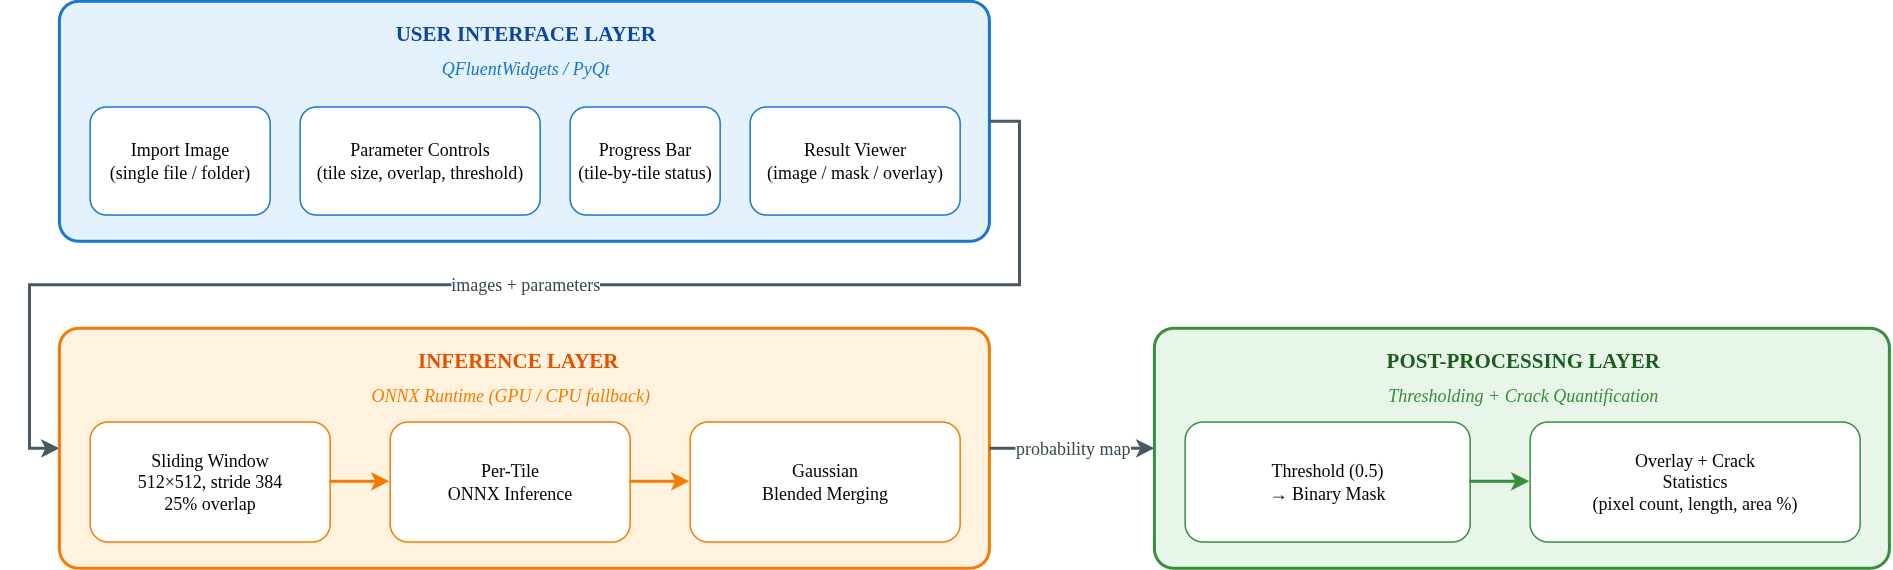
\includegraphics[width=\linewidth]{figures/application/application-architecture.png}
    \caption{\textit{Three-layer architecture of the desktop inspection application..}}
    \label{fig:application_architecture}
\end{figure}

\hs Images flow from the user interface through the ONNX-based inference layer, where sliding-window tiling and Gaussian blended merging are applied, to the post-processing layer that produces binary crack masks and quantitative statistics.

\textbf{Workflow.} The user workflow consists of four steps:

\begin{enumerate}
    \item Import a UAV image (single file or folder batch).

    \item Configure inference parameters (tile size default: 512×512; overlap default: 128 px; threshold default: 0.5).

    \item Run inference, the app displays a progress bar and processes tiles sequentially on the available GPU/CPU.

    \item View results, the app shows the original image, binary mask, overlay, and a summary panel with crack overlay.
\end{enumerate}

\textbf{Deployment Target.} The application is designed for desktop deployment on inspection workstations and field laptops. It supports both GPU (CUDA via ONNX Runtime) and CPU fallback, ensuring operability on machines without dedicated graphics hardware. The ONNX export described in Section \ref{subsec:model_export} ensures that the app does not require a PyTorch installation, reducing deployment size and dependency conflicts.